%%% Local Variables: 
%%% mode: latex
%%% TeX-master: "../KanjiHWR"
%%% End: 

\chapter{Technical Design of the Application}
\label{chap:technicaldesign}

The focus of this chapter is on the general architectural choices made during
the development of the system. In this chapter, the technical design aspects 
of the application are described. The general system architecture is layed out in
section~\ref{sec:systemarchitecture}. It contains the global view on the software
architecture in section~\ref{sec:globalarchitecture}, the data flow in within
the system in section~\ref{sec:arch:systemdataflow} and describes the design
of the individual modules in section~\ref{sec:arch:softwaremodules}.
Section~\ref{sec:frameworkanddevices} describes the technical set-up and 
framework choices. However, the handwriting recognition engine is described 
in detail in a separate 
section~(see chapter~\ref{chap:handwritingrecognitionengine}).

\section{System Architecture}
\label{sec:systemarchitecture}

The system architecture of the Kanji Coach follows the requirements of an 
e-learning environment dealing with the specific difficulties for learners 
of the Japanese script (see chapter~\ref{chap:japanasescript}) and those of an 
on-line handwriting recognition. Techniques of handwriting recognition are 
reviewed in chapter~\ref{chap:onlinehwr}. The general requirements of an 
e-learning application are presented in chapter~\ref{chap:elearning}. 
The resulting specific conceptual design choices have been 
layed out in chapter~\ref{chap:conceptualdesignofkanjicoach}. This
section deals with the technical aspects of the system design.

\subsection{Global Architecture}
\label{sec:globalarchitecture}

The global architecture of the application follows the Model-View-Controller
(MVC) design pattern. This paradigm is used as a general model, however, 
it is not designed the strict way proposed by~\shortcite{Krasner1988}.
Figure~(\ref{fig:modelviewcontroller}) shows the general set-up of the 
MVC design pattern after~\shortcite{Krasner1988}. xxx: Also 
figure~(\ref{fig:modelviewcontroller2}) - decide how it should be done and use
the appropriate gfx. xxx!
In the MVC paradigm the \emph{model} is a domain-specific software, 
an implementation of the central structure of the system. It can be a simple
integer, representing a counter or it could be a higly complex object structure, 
even a whole software module. The \emph{view} represents anything graphical. 
It requests data from the model and displays the result. The \emph{controller} 
is the interface between the model and the view. It controls and scheduls the 
interaction between the input devices, the model and the 
view~\shortcite{Krasner1988}.
%xxx Make this a graphic, not a photographic image of a graphic 
\begin{figure}[htbp]
\begin{center}
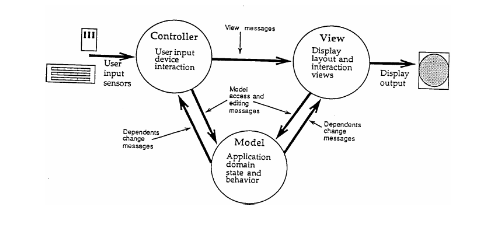
\includegraphics[scale=0.5]{images/TechnicalDesign/MVC.png}
\caption{The Model-View-Controller paradigm}
\label{fig:modelviewcontroller}
\end{center}
\end{figure}

%xxx Make this a graphic, not a photographic image of a graphic 
\begin{figure}[htbp]
\begin{center}
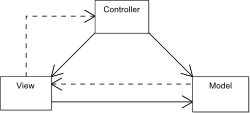
\includegraphics[scale=0.5]{images/TechnicalDesign/ModelViewControllerDiagram.png}
\caption{The Model-View-Controller paradigm AGAIN!}
\label{fig:modelviewcontroller2}
\end{center}
\end{figure}

A global overview of the system architecture can be seen in 
figure~(\ref{fig:globalarchitecture}).
%xxx Make this a graphic, not a photographic image of a graphic 
\begin{figure}[htbp]
\begin{center}
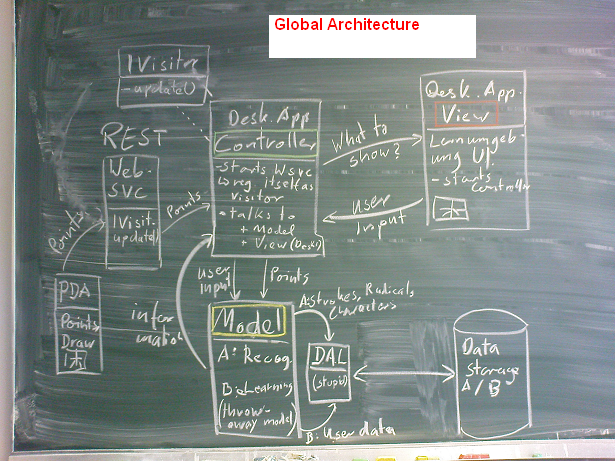
\includegraphics[scale=0.5]{images/TechnicalDesign/GlobalArchitecture.png}
\caption{The global architecture of the software system}
\label{fig:globalarchitecture}
\end{center}
\end{figure}

\subsection{System Data Flow}
\label{sec:arch:systemdataflow}
The system data flow is shown in figure~(\ref{fig:systemdataflow}).
%xxx Make this a graphic, not a photographic image of a graphic 
\begin{figure}[htbp]
\begin{center}
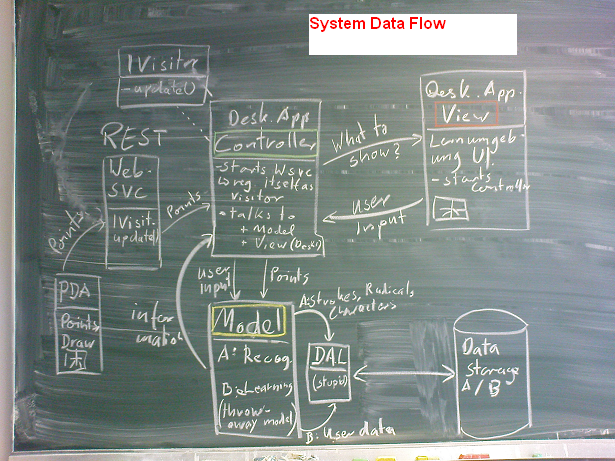
\includegraphics[scale=0.5]{images/TechnicalDesign/SystemDataFlow.png}
\caption{The data flow within the software system}
\label{fig:systemdataflow}
\end{center}
\end{figure}
The controller lies in the centre of the application, it runs on the stationary
device. It contains a web service that is used as an interface to receive data 
from the handwriting input data view. The desktop view is the main interaction 
point for the user. The model contains the logic, while the data access layer 
provides a reusable interface for storing data. The details of 
figure~(\ref{fig:systemdataflow}) are described in subsequent 
sections~\ref{sec:arch:recognitiondataflow} and~\ref{sec:arch:learningdataflow}.

\subsubsection{Communication}
\label{sec:communication}

The communication between the different parts of the application is realised 
in two independet and distinct ways. The communication between the 
modules running under the same process is realised via a messaging system. 
The communication between the modules that run on different devices
or at least as a separate process is realised via a web service.

\emph{Loose coupling} is used here as a term to emphasize that different modules 
in a larger system are only loosely connected and do not depend largely on each 
other. \emph{Coupling} can be understood as the degree of knowledge a module or 
class have of each another. The lesser the knowledge of each other the software 
modules can manage with, the more loose the coupling.

In the course of the design and development cycles of the Kanji Coach, 
it became apparent that it has to be possible to attach different views, 
input devices and data storage systems to the controller. This is due to the 
distributed nature of the application. 
In order to ensure that the handwriting data input view, which currently runs 
on a mobile device, can run on a different device, it had to be loosly coupled 
to the main controller. Therefore, the communication between the handwriting 
input data view and the main controller is realised via a web service. 
Because of this communication structure, it is possible to exchange the 
handwriting data input view with a different one, for instance when running 
the application on a device like a tablet PC. The design of the communication 
structure within the web service is described in greater detail 
in section~\ref{sec:arch:webservice}.

The messaging system that forms the communication structure between the software 
modules running as the same process is realised with a message class that
can be manipulated by the modules using these messages.
Technically, the web service and the controller both run as a subprocess of the 
main desktop view. When the web service receives a request and accompanying data
from the handwriting input data view, both request and data are bundled into an 
encapsulated message and passed to the controller. A similar type of message 
is used for requests from the controller to the model, for instance a recognition
task that needs be performed.

\subsubsection{Recognition Data Flow}
\label{sec:arch:recognitiondataflow}

The recognition data flow is simply the flow of data occuring in a recognition 
scenario. It can be described in \ref{recdataflowDisplayResult} steps
as depicted in figure~(\ref{fig:systemdataflow}).
\begin{enumerate}
  \item \label{recdataflowClear} 
        Clearing the input GUI screen 
        [Controller $\Rightarrow$ Web service $\Rightarrow$ Handwriting data input view]
  \item \label{recdataflowTransmit} 
        Transmitting user input data to the web service 
        [Handwriting data input view $\Rightarrow$ Web service]
  \item \label{recdataflowEncapsulatePass} 
        Encapsulating data into a message and passing 
        it to the controller 
        [Web service $\Rightarrow$ Controller]
  \item \label{recdataflowRequestRecognition} 
        Requesting recognition 
        [Controller $\Rightarrow$ Model] 
  \item \label{recdataflowReturnResult} 
        Returning recognition result 
        [Model $\Rightarrow$ Controller] 
  \item \label{recdataflowDisplayResult} %this should be the last label, otherwise seek for the place where it is used as a number and change it to the new last label there
        Displaying recognition result 
        [Controller $\Rightarrow$ Desktop view]
\end{enumerate}
When the desktop application requests the use to input a Kanji 
character, it sends a message to the web service advising the handwriting data 
input view to clear the screen (step~\ref{recdataflowClear}). 
The handwriting data input view receives the information by polling the web 
service. 
When the user starts drawing on the surface of the handwriting data input view, 
the data is caputered and transmitted to the web service 
(step~\ref{recdataflowTransmit}).
Each stroke is captured and sent individually in order to ensure a faster 
recognition. That way, the recognition process is initiated before the
user finishes writing a character. The web service receives the data and 
creates an encapsulated message. That message is passed to the 
controller (step~\ref{recdataflowEncapsulatePass}).
The controller initiates a request to the model, containing all strokes
subsequent to the last clear screen 
event (step~\ref{recdataflowRequestRecognition}).
The model performs the recognition of the set of strokes and returns the result
or partial result to the controller (step~\ref{recdataflowReturnResult}).
The controller advises the desktop view to display the resulting character
(step~\ref{recdataflowDisplayResult}).

\subsubsection{Learning Data Flow}
\label{sec:arch:learningdataflow}

The learning data flow is the data flow between the learning module of the 
application, the recognition process and the user interaction.
The learning data flow design can be summed up 
in~\ref{learningdataflowDisplayLearningState} steps.
\begin{enumerate}
  \item \label{learningdataflowAskForDrawing} 
        In learning mode or test mode: Asking user to draw a character,
        based on the current lesson data. The controller sends a display
        request to the desktop view.
        [Controller $\Rightarrow$ Desktop view]
  \item \label{learningdataflowRequestStoring} 
        After recognition process: Request storing recognised character in 
        learning profile.
        [Controller $\Rightarrow$ Model]
  \item \label{learningdataflowStoring} 
        Calculation of error points for a character (creation of new data) and
        storage.
        [Model $\Rightarrow$ Data access layer]
  \item \label{learningdataflowReturningLearningState} 
        Returning learning state of character 
        [Model $\Rightarrow$ Controller] 
  \item \label{learningdataflowDisplayLearningState} %this should be the last label, otherwise seek for the place where it is used as a number and change it to the new last label there
        Displaying learning state 
        [Controller $\Rightarrow$ Desktop view
\end{enumerate}
The learning data flow is described in the middle of a user interaction with the
learning application as it illustrates a typical data flow most appropriately
as shown in figure~(\ref{fig:systemdataflow}).

In step~\ref{learningdataflowAskForDrawing} of the learning data flow, the 
controller sends a message to the desktop view with a request to display an 
invitation to the user to draw a specific character.
That step is a part of the general messaging system design that manages the 
communication between the controller and the other modules.
When the recognition process is finished, the character needs to be stored.
The controller requests the model to store the 
character (step~\ref{learningdataflowRequestStoring}).
The logic layer then creates new data, namely the error points of a 
character that naturally become a part of the data flow.
Both the character recognition result and the error points are stored
using the data access layer (step~\ref{learningdataflowStoring}). 
The resulting learning state defines which character will be displayed next.
This calculation result is transmitted from the model to the 
controller after storage in the penultimate 
step~(\ref{learningdataflowReturningLearningState}).
The last step in the learning data flow is the display of the resulting learning 
state to the user in the desktop 
view (step~\ref{learningdataflowDisplayLearningState}).

\subsection{Software Modules}
\label{sec:arch:softwaremodules}

\subsubsection{Handwriting Data Input View}
\label{sec:arch:handwritingdatainputview}

%Put a gfx with a screen shot here.
%http://kleineurl.de/1kfec2.htm
%http://kleineurl.de/1kfeav.htm
%http://kleineurl.de/1kfebg.htm
%http://kleineurl.de/1kfebt.htm
%http://kleineurl.de/1kfecf.htm
%http://kleineurl.de/1kfecs.htm

The handwriting data input view is a graphical user interface. It is designed for
simplicity and usability. It's main task is data capturing.
It contains only an input area, with a cross in order for the user to better 
locate the strokes of the character. This follows a common practice in Kanji 
teaching - a cross departs the writing area in four areas.

There is no \emph{commit} or \emph{finish} button on the handwriting data 
input GUI, since the end of a stroke sequence is handled with a time out in 
the learning module. When the user needs too long to input a character there 
is a problem and help should be offered.
Therefore, it is sufficient to only display a reset button on the writing area.
Whenever the reset button is pressed, the controller is notified of that event.
The current drawing will be removed from the screen. The next user input will
be treated as a new character

In the background of the handwriting data input view the user input is sent to 
the controller module. Besides that, a polling mechanism ensures that any 
messages from the controller to the handwriting input data view are received.
Whenever the user finishes a stroke, the module sends a message via a web service
(see section~\ref{sec:arch:webservice}) to the controller.

\subsubsection{Main View}
\label{sec:arch:mainview}

%xxx graphic of UI design here, maybe a sketch and maybe a screenshot.
The main view of the system is a graphical user interface. It contains a simple
learning environment, a display area for the characters that have been drawn
in the handwriting input area an information area that displays addidional 
information about a character. In a configuration area the user can choose 
between the different lessons the system offers and between a training mode
and a test mode.

\subsubsection{Web Service}
\label{sec:arch:webservice}

The main communication module between the handwriting data input view and the 
controller is a web service that runs on the main part of the application
as a subprocess of the controller. When the desktop application requests the 
user to input a Kanji character, it sends a message to the web service 
advising the handwriting data input view to clear the screen. 
The handwriting data input view receives the information by polling the 
web service. However, the main task of the web service is to receive data 
from the handwriting input data view and forward that data to the controller
of the system.
\shortcite{W3C1997}

http://de.wikipedia.org/wiki/Windows_Communication_Foundation
http://en.wikipedia.org/wiki/Web_service
http://kleineurl.de/1kfd1k.htm


\subsubsection{Recognition Module}
\label{sec:arch:recognitionmodule}

\subsubsection{Learning Module}
\label{sec:arch:learningmodule}

\section{Framework and Devices}
\label{sec:frameworkanddevices}

\subsection{Operating System}
\label{sec:operatingsystem}

\subsection{Framework}
\label{sec:framework}

http://de.wikipedia.org/wiki/Windows_Communication_Foundation

.NET vs. Java etc.

\subsection{Desktop Computer}
\label{sec:desktopcomputer}

\subsection{Pen Input Device}
\label{sec:peninputdevice}

warum mobil? - damit man sehen kann, was man macht!

\subsubsection{Stylus Input}
\label{sec:stylusinput}

